% First differences of f(n)=n^2/20. Circle angles: 0, 18, 72, 162, 288, 90, 288 degrees.
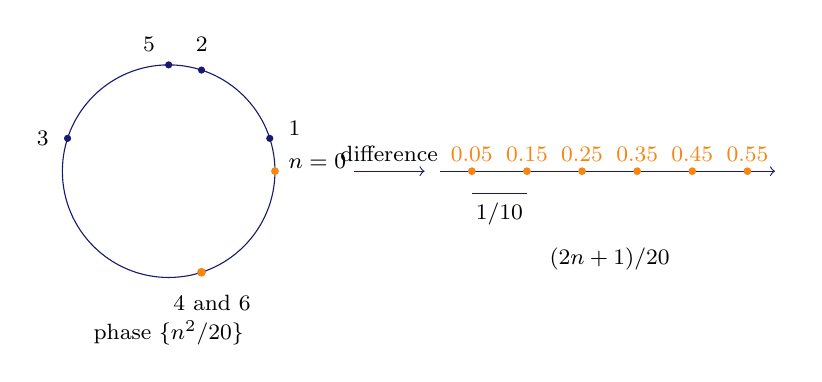
\begin{tikzpicture}[every node/.style={font=\footnotesize}]
  \draw[MidnightBlue] (0,0) circle (1.35);
  \fill[BurntOrange] (1.35,0) circle (1.4pt);
  \node[right] at (1.40,0.12) {$n=0$};
  \fill[MidnightBlue] (1.284,0.417) circle (1.3pt);
  \node[right] at (1.40,0.55) {$1$};
  \fill[MidnightBlue] (0.417,1.284) circle (1.3pt);
  \node[above] at (0.42,1.40) {$2$};
  \fill[MidnightBlue] (-1.284,0.417) circle (1.3pt);
  \node[left] at (-1.40,0.42) {$3$};
  \fill[MidnightBlue] (0,1.35) circle (1.3pt);
  \node[above left] at (-0.05,1.40) {$5$};
  \fill[BurntOrange] (0.417,-1.284) circle (1.6pt);
  \node[below] at (0.55,-1.45) {$4$ and $6$};
  \node at (0,-2.05) {phase $\{n^2/20\}$};

  \draw[MidnightBlue,->] (2.35,0)--(3.25,0);
  \node[above] at (2.80,0) {difference};

  \draw[MidnightBlue,->] (3.45,0)--(7.7,0) node[below right] {};
  \fill[BurntOrange] (3.85,0) circle (1.4pt) node[above] {$0.05$};
  \fill[BurntOrange] (4.55,0) circle (1.4pt) node[above] {$0.15$};
  \fill[BurntOrange] (5.25,0) circle (1.4pt) node[above] {$0.25$};
  \fill[BurntOrange] (5.95,0) circle (1.4pt) node[above] {$0.35$};
  \fill[BurntOrange] (6.65,0) circle (1.4pt) node[above] {$0.45$};
  \fill[BurntOrange] (7.35,0) circle (1.4pt) node[above] {$0.55$};
  \draw[MidnightBlue] (3.85,-0.28)--(4.55,-0.28);
  \node[below] at (4.20,-0.28) {$1/10$};
  \node[below] at (5.6,-0.85) {$(2n+1)/20$};
\end{tikzpicture}
